Previous chapters introduced some of the fundamental concepts related to robotic perception, and specifically techniques for sensing the environment and extracting useful semantic information. While these techniques provide \textit{local} information that is crucial for robots to navigate autonomously, additional \textit{global} information is often required. 
For example, distance measurements from a laser rangefinder might be useful for detecting objects in an environment, but they only provide information \textit{relative} to the robot's current position. Alternatively, object detection via computer vision only provides information about what is in the robot's \textit{current} view. Robotic autonomy, in particular autonomous decision making and planning, generally requires more than just local information to answer questions such as ``have I seen this object before?'' and ``have I been here before?''.
These new challenges, associated with building a global understanding of the environment from local measurements, are often referred to as \textit{localization and mapping}\footnote{Localization and mapping is the component of the ``think'' part of the ``see, think, act'' cycle that connects with robotic perception.}.


\notessection{Introduction to Localization and Filtering}


The problem of \textit{localization} is to endow the robot with the ability to understand its current position with respect to its environment in a global sense\cite{ThrunBurgardEtAl2005}\cite{SiegwartNourbakhshEtAl2011}.
One of the main classes of techniques for robot localization are \textit{map-based}, where the robot explicitly localizes its position with respect to a \textit{map} of the environment.
For example, consider the floor plan (the environment map) in Figure \ref{fig:sample-room}: before a robot can navigate to a particular room it must know where in the building it is currently located.\footnote{Other approaches to navigate in environments include \textit{behavioral} approaches, which rely on a specified set of behaviors that will result in a desired global behavior without the need for explicit mapping or localization. An example of this approach would be to have a left-wall following behavior for movement about a building.}
\begin{figure}[ht]
	\centering
    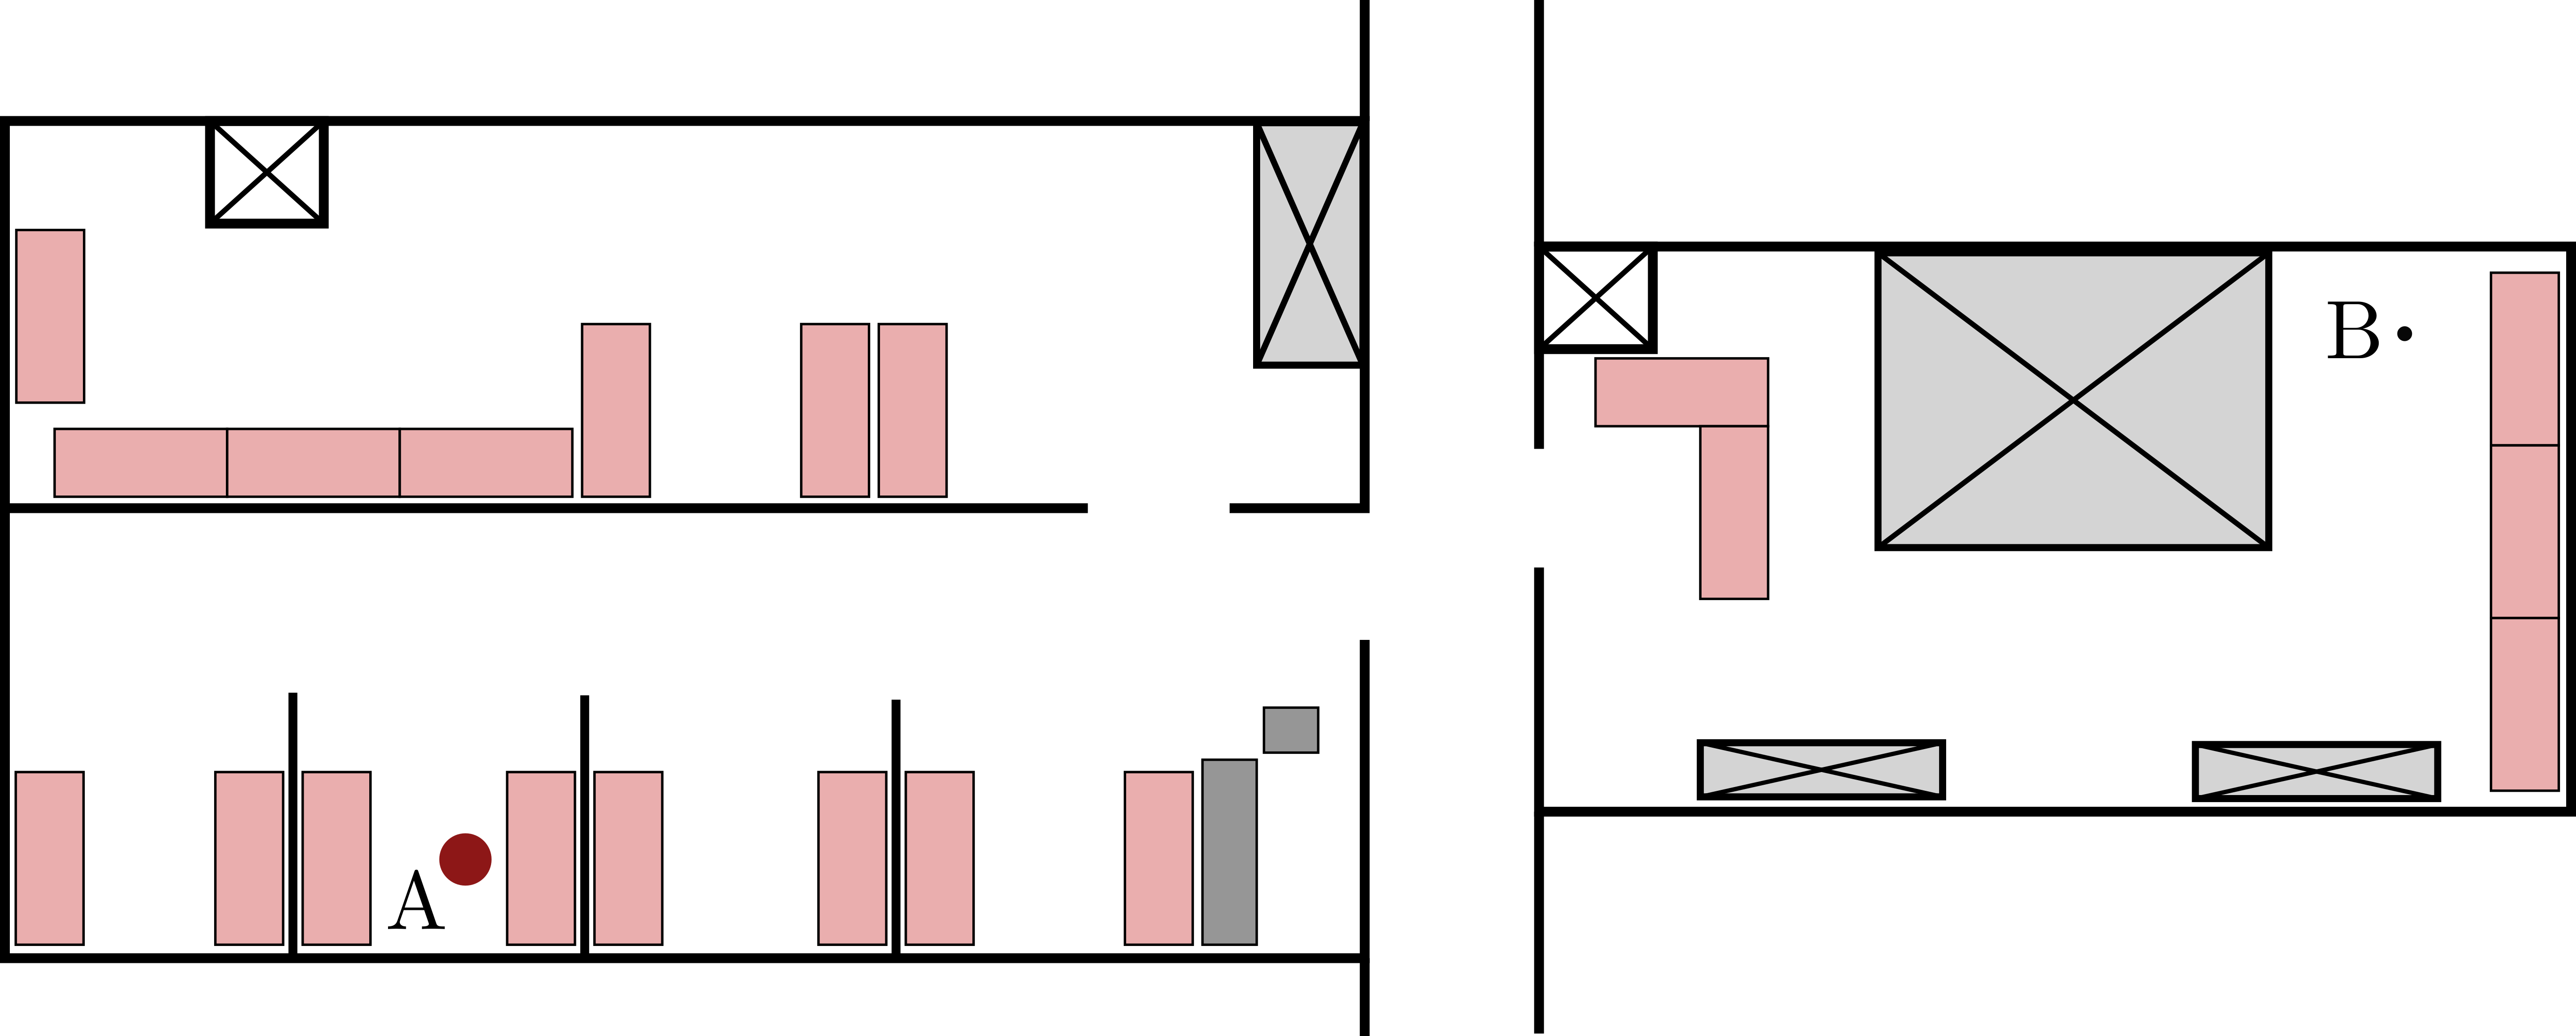
\includegraphics[width=0.9\textwidth]{tex/figs/ch14_figs/map.png}
    \caption{An example environment where localization is crucial for robotic autonomy. For a robot to move from location A to location B it must first understand which room it is in, and that the only path to B is through the hallway. Extracting such global information about the environment from local measurements (e.g. from a range sensor) requires specialized algorithms.}
    \label{fig:sample-room}
\end{figure}

There are two primary components to map-based localization: map representation and belief representation. This chapter focuses on belief representation, which addresses the problem of how to best represent the robot's belief of its current position with respect to the map. One simple approach would be to simply store a best guess of the robot's position (in some map-based coordinate system). However in practice localization information is often \textit{uncertain}, and representing the belief by only a best guess does not capture this important fact. Therefore one common approach is to use a \textit{probabilistic} representation of the robot's belief since probability distributions can be used to model uncertainty (and extract best guesses, for example by finding the mean of a unimodal distribution). A variety of probabilistic representations can be used, for example singe-hypothesis or multiple-hypothesis representations as well as continuous or discrete representations. A few examples showing the differences between these types of representations are given in Figure \ref{fig:belief-representation}.
\begin{figure}[ht!]
	\centering
    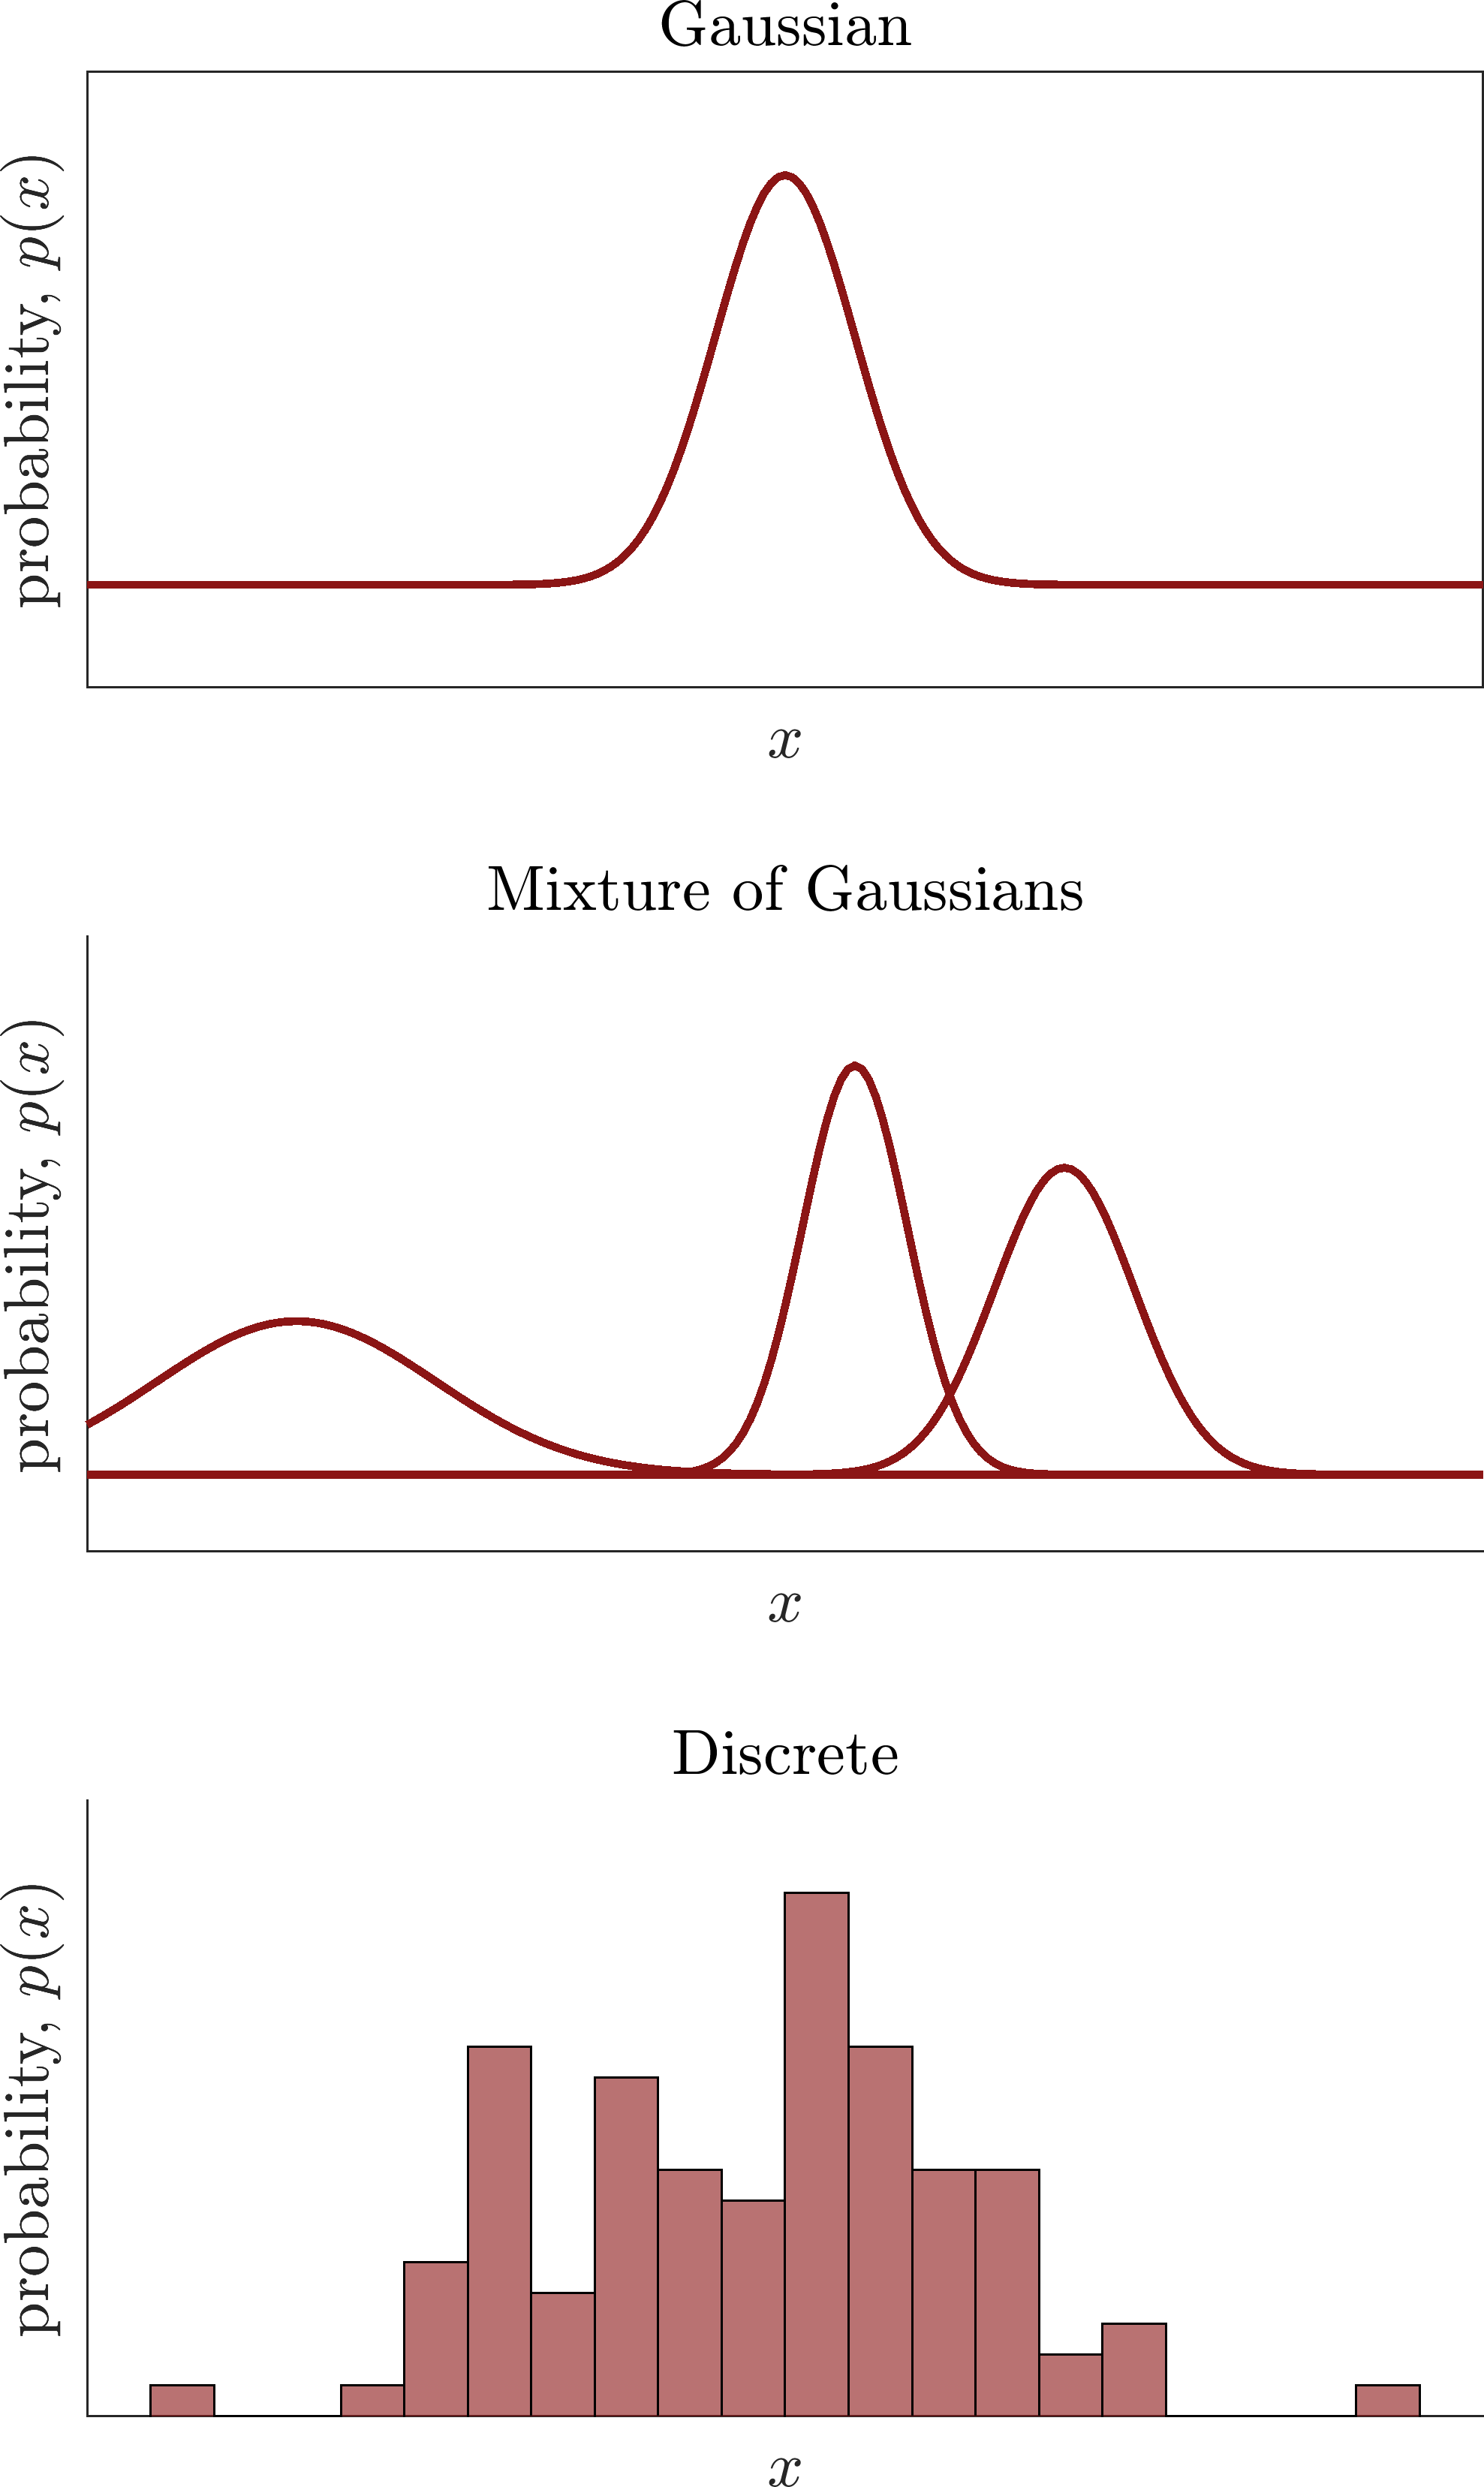
\includegraphics[width=0.6\textwidth]{tex/figs/ch14_figs/distributions.png}
    \caption{A graphical representation of different types of probabilistic representations: (a) a continuous single-hypothesis belief (e.g. from a single Gaussian distribution), (b) a continuous multiple-hypothesis belief (e.g. a mixture of Gaussians), (c) discrete representation with a finite number of possible values.}
    \label{fig:belief-representation}
\end{figure}
Some representations are more expressive than others, but there is usually a trade-off with computational complexity of the resulting algorithms that support the representation. Algorithms based on these different probabilistic representations will be presented in this chapter and in subsequent chapters.

\subsection{Basic Concepts in Probability}
Before discussing different types of robot localization algorithms it is useful to provide a review of some of the fundamental concepts from probability. 

\subsubsection{Random Variables}
Uncertain quantities such as sensor measurements, robot state, and environment variables can be modeled as discrete or continuous \textit{random variables}.
\begin{definition}[Discrete Random Variable]
A discrete random variable $X$ is a random variable that can only take on values from a countable set. Discrete random variables are characterized by a probability mass function $p(x)$ (which can be read as $p(X=x)$, ``the probability that $X$ takes on value $x$'') that satisfies:
\begin{equation*}
    \sum_x p(x) = 1,
\end{equation*}
where the summation is over all possible values of $X$.
\end{definition}
\begin{definition}[Continuous Random Variable]
A continuous random variable $X$ is a random variable that can take on values from a continuous range. Continuous random variables are characterized by a probability density function $p(x)$ that satisfies:
\begin{equation*}
    \int_{-\infty}^\infty p(x) dx = 1.
\end{equation*}
The probability of the random variable taking on a value in the interval $[a,b]$ is similarly defined as:
\begin{equation*}
    P(a \leq X \leq b) = \int_{a}^b p(x) dx = 1.
\end{equation*}
\end{definition}
A common example of a discrete random variable is the result of a coin flip, which can only take on two values: heads or tails. In robotics, a common example of a continuous random variable may be the position of the robot, which could take on an infinite number of values.

\subsubsection{Joint Distributions, Independence, and Conditioning}
Many applications of probability theory rely on more than one random variable. In these instances it is useful to be able to quantify probabilities associated with multiple random variables at the same time. One of the most fundamental tools when dealing with multiple variables is the \textit{joint distribution}.
\begin{definition}[Joint Distribution]
The joint distribution of two random variables $X$ and $Y$ defines the probability associated with both taking on specific values at the same time. This is denoted mathematically as $p(x,y)$, which can be read as $p(X=x \:\:\text{and}\:\: Y=y)$.
\end{definition}
It is also useful to determine whether different random variables have any relationship to each other. In particular, two random variables that do not have any influence on each other in a probabilistic sense are considered to be probabilistically independent.
\begin{definition}[Independence]
Two random variables $X$ and $Y$ are independent if and only if:
\begin{equation} \label{eq:indep}
    p(x,y)=p(x)p(y).
\end{equation}
Independence holds when the occurrence of one value of a random variable does not affect the probability of another random variable taking on a specific value.
\end{definition}
Another useful tool that relates two random variables is the conditional probability, which defines the probability of a random variable when the value of a second random variable is \textit{known} or \textit{fixed}.
\begin{definition}[Conditional Probability]
The conditional probability of a random variable $X$ taking on a value given that a second random variable $Y$ has a specific value is defined as:
\begin{equation} \label{eq:condprob}
    p(x\:|\: y)\coloneqq \frac{p(x,y)}{p(y)}.
\end{equation}
This can be read as ``the probability of $X$ taking on value $x$ conditioned on the fact that $Y$ has taken on value $y$''.
\end{definition}
Notice that if the random variables $X$ and $Y$ are independent, then the conditional probability definition simplifies to $p(x\:|\: y) = p(x)$, which suggests that knowing that $Y$ has taken on value $y$ has provided no new information about the random variable $X$ (which of course is in line with the definition of independence).
Additionally, another notion of independence can be defined based on whether or not two random variables are independent when \textit{conditioned} a third random variable.
\begin{definition}[Conditional Independence]
Two random variables $X$ and $Y$ are conditionally independent given the value of a third random variable $Z$ if and only if:
\begin{equation} \label{eq:condindep}
    p(x,y\:|\: z) = p(x \:|\: z) p(y \:|\: z).
\end{equation}
\end{definition}
It is important to note however that conditional independence does not imply independence, and vice versa.

\subsubsection{Law of Total Probability}
The law of total probability defines a relationship between probabilities, joint probabilities, and conditional probabilities.
\begin{definition}[Law of Total Probability]
For discrete random variables $X$ and $Y$ the law of total probability states that:
\begin{equation*}
    p(x) = \sum_y p(x,y) = \sum_y p(x \:|\: y) p(y). 
\end{equation*}
Similarly, for continuous random variables this law is given by:
\begin{equation*}
    p(x) = \int p(x,y) dy = \int p(x \:|\: y) p(y) dy. 
\end{equation*}
\end{definition}
In words, this law says that the probability of a random variable $X$ taking on a value $x$ can be found by looking at the joint probabilities between $X$ and $Y$ and accounting for \textit{all} possible values of $Y$. The second part of the law is a direct result of applying the definition of conditional probabilities.

\subsubsection{Bayes' Rule}
The joint probability $p(x,y)$ between two random variables $X$ and $Y$ can be related to the conditional probabilities $p(x \:|\: y)$ and $p(y \:|\: x)$ via the definition of conditional probabilities \eqref{eq:condprob}. In particular, since the joint probability can be equivalently expressed in two ways it can be seen that:
\begin{equation*}
    p(x,y) = p(x \:|\: y)p(y) = p(y \:|\: x) p(x).
\end{equation*}
This relationship is commonly referred to as Bayes' rule:
\begin{definition}[Bayes' Rule]
For discrete random variables $X$ and $Y$, Bayes' rule states that:
\begin{equation} \label{eq:bayes}
    p(x \:|\: y) = \frac{p(y \:|\: x) p(x)}{p(y)}. 
\end{equation}
\end{definition}
Bayes' rule is useful as it provides a relationship between the ``inverse'' conditional probabilities $p(x \:|\: y)$ and $p(y \:|\: x)$. This is particularly important for \textit{probabilistic inference}, which is the problem of inferring the value of a random variable from another. 

For example, suppose you had a good initial guess of the probability distribution $p(x)$ for a random variable $X$ (the distribution $p(x)$ in this case is often called the \textit{prior}, because it is the guess that comes before any new information is taken into account). Then, suppose some new information regarding the value of a random variable $Y$ is obtained. Using Bayes' rule it is possible to update your belief about the probability distribution of $X$ based on this new information. In particular, the new belief is the conditional probability $p(x \:|\: y)$ (which is often called the \textit{posterior} because it comes after new information is introduced). These two distributions are related by Bayes' rule!

Bayes' rule can also be extended to cases with additional random variables. For example with three random variables $X$, $Y$, and $Z$, Bayes' rule is:
\begin{equation*}
    p(x \:|\: y, z) = \frac{p(y \:|\: x, z) p(x \:|\: z)}{p(y \:|\: z)}. 
\end{equation*}

\subsubsection{Expectation and Covariance}
Probability distributions define in a vary precise way the probability associated with any particular value of a random variable. However, sometimes it is useful to aggregate this information into more practically useful metrics. Two of the most commonly used metrics are the \textit{expected value} and the \textit{covariance}.
\begin{definition}[Expected Value]
The expected value for a random variable $X$ is denoted as $E[X]$. For discrete random variables the expected value can be computed by:
\begin{equation*}
    E[X] = \sum_x x p(x).
\end{equation*}
Similarly, the expected value for a continuous random variable can be computed by:
\begin{equation*}
    E[X] = \int x p(x) dx.
\end{equation*}
\end{definition}
The expected value can be thought of as the average result of an experiment over an infinite number of trials, and is also sometimes referred to as the \textit{first moment} of the distribution.
Additionally, expectation is a \textit{linear operator}, such that:
\begin{equation*}
    E[aX + b]= aE[X] + b,
\end{equation*}
for any values $a$ and $b$.
In the case that the random variable $X$ is a vector-valued random variable, the expectation of the random vector is simply the vector of expectations of each element.

\begin{definition}[Covariance]
The covariance between two random variables $X$ and $Y$ is denoted $\text{cov}(x,y)$ and is computed by:
\begin{equation*}
    \text{cov}(x,y) = E[(X-E[X])(Y-E[Y])^T] = E[XY^T] - E[X]E[Y]^T
\end{equation*}
\end{definition}
Covariance is a metric used to describe the relationship between random variables and is positive if greater values of one variable generally corresponds to greater values of the other (and same for lesser values). Similarly, it is negative if the variables tend to show opposite behavior of each other. If there is no general relationship between the two then their covariance is zero (e.g. independent random variables have zero covariance).


\subsection{Markov Models}
Recall from previous chapters the kinematic and dynamic models that were developed to describe the physical behavior of a robot. These models consisted of a robot state $\x$, and a set of equations that described how $\x$ varied in time given some control inputs $\bu$. In this section another type of model will be developed that is based on these same core ideas. These new models, referred to as \textit{Markov models}, are commonly used in robotics for localization tasks as well as higher level planning tasks.

\subsubsection{States, Measurements, and Controls}
Similar to previous chapters, the state $\x$ is a collection of variables that contains information required to define the physical state of the robot. However unlike previous chapters, the state might also include information about the environment (this state has a higher-level perspective). In the context of robotics, the state may include the robot pose (i.e. location and orientation information), velocity, as well as locations and features of surrounding objects in the environment. 
Note that in general the state discussed in this section might be different from the state defined for robot kinematics and dynamics (even if the robot is the same). This is because the choice of model is usually specific to the task at hand, and while the kinematic and dynamic models are useful for control, they may not strictly be necessary (or sufficient) for use in localization and planning tasks.

A discrete time formulation is also used in this context, where the state is specified for discrete time instances and denoted by $\x_t$ (rather than $\x(t)$, as was done in previous chapters). The models developed in this section then describe the changes in the state between time steps, for example between $\x_t$ and $\x_{t+1}$. It is also useful to define the notation $\x_{t_1:t_n} \coloneqq \x_{t_1},\x_{t_2},...,\x_{t_n}$ for describing a sequence of states between times $t_1$ and $t_n$.

The robot interacts with the environment through control actions and by gathering information through measurements\footnote{In the context of robot localization, measurements increase the robot's knowledge and control actions tend to result in a loss of knowledge.}. In this context, the measurement data collected at a time $t$ will be denoted as $\z_t$, and the control data is denoted as $\bu_t$. Similar to the state, a useful notation for representing a sequence of measurements or controls is given by  $\z_{t_1:t_n} \coloneqq \z_{t_1},\z_{t_2},...,\z_{t_n}$ and $\bu_{t_1:t_n} \coloneqq \bu_{t_1},\bu_{t_2},...,\bu_{t_n}$. In general, the measurements can come from any number of the sensors discussed in previous sections on robotic perception, including cameras and laser rangefinders.

\subsubsection{Model}
The kinematic and dynamic models from previous chapters (expressed as a set of ordinary differential equations) were deterministic models. However, to leverage a probabilistic framework for robot localization it is typically required that the model also be probabilistic. In the most general sense a probabilistic model can be defined by:
\begin{equation} \label{eq:genprobmod}
p(\x_t \mid \x_{0:t-1}, \z_{1:t-1}, \bu_{1:t}),
\end{equation}
which defines a probability distribution over the possible current state $\x_t$ given the state, measurement, and control histories. Note that here the convention that will be used is that the robot executes control $\bu_t$ first, and then the measurement $\z_t$ can be made based on the resulting state $\x_t$. A general probabilistic measurement model can also be defined as:
\begin{equation} \label{eq:genmeasmod}
p(\z_t \mid \x_{0:t}, \z_{1:t-1}, \bu_{1:t}).
\end{equation}

In many cases however, the state is defined such that it is \textit{complete}. A state $\x_t$ is complete if no variables prior to $\x_t$ can influence the future states. In other words, $\x$ contains a sufficient amount of information that the history is not important. This is also known as the \textit{Markov property}. If the Markov property holds, the probabilistic model \eqref{eq:genprobmod} can be simplified to:
\begin{equation} \label{eq:markovprobmod}
p(\x_t \mid \x_{t-1}, \bu_{t}),
\end{equation}
and the measurement model \eqref{eq:genmeasmod} can be simplified to:
\begin{equation} \label{eq:markovmeasmod}
p(\z_t \mid \x_{t}).
\end{equation}

The resulting overall model with the Markov property, consisting of the state transition probability \eqref{eq:markovprobmod} and the measurement model \eqref{eq:markovprobmod} is referred to as a Bayes network model or a hidden Markov model. Graphically this model can be represented as shown in Figure \ref{fig:hmm}, where the sequencing of the control and measurements are more clearly shown (first control, then measurement).
\begin{figure}[ht]
	\centering
    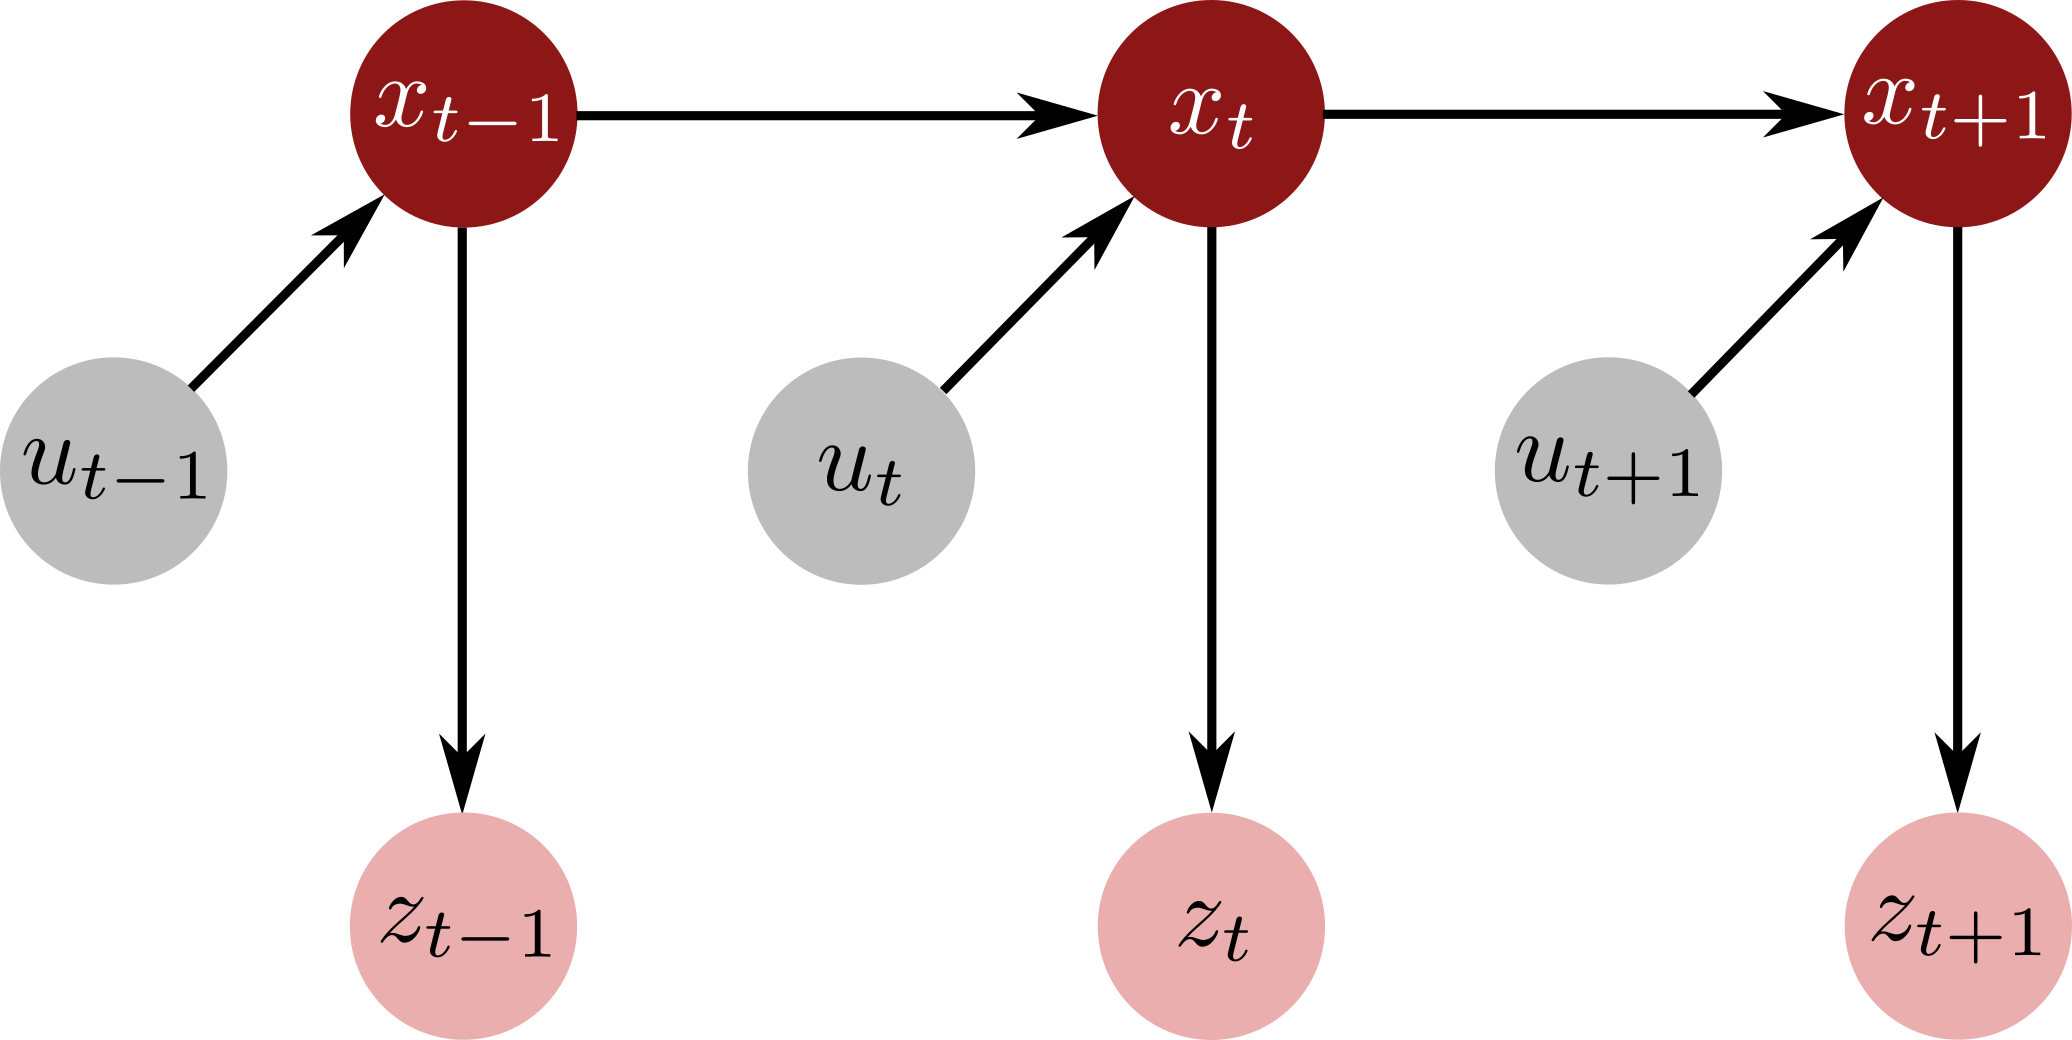
\includegraphics[width=0.55\textwidth]{tex/figs/ch14_figs/hmm.png}
    \caption{Graphical representation of the Bayes network model (hidden Markov model). Note that the sequencing assumes that the control is applied, and then a measurement is taken.}
    \label{fig:hmm}
\end{figure}


\subsection{Bayes Filter}
Given a Bayes network model defined by a state transition model \eqref{eq:markovprobmod} and a measurement model \eqref{eq:markovmeasmod}, the next task is to determine a way to use this information for robot localization. In particular, the desired task is to estimate the current robot state $\x_t$ given the measurement and control information that is available. In the probabilistic framework this estimate is referred to as a \textit{belief distribution}, which is a probability distribution over $\x$. This distribution assigns a probability to each hypothesis with respect to the true state. Mathematically the belief distribution is denoted as $bel(\x_t)$ and is defined as:
\begin{equation} \label{eq:belief}
bel(\x_t):=p(\x_t\mid \z_{1:t}, \bu_{1:t}).
\end{equation}
In other words, the belief $bel(\x_t)$ is a posterior probability distribution over the state variables conditioned on the available data. A similar distribution, known as the \textit{prediction} distribution, can also be defined as:
\begin{equation} \label{eq:predbelief}
\overline{bel}(\x_t):=p(\x_t\mid \z_{1:t-1},\bu_{1:t}),
\end{equation}
which is does not include the most recent measurement $\z_t$. The process of computing a belief from a predicted belief (i.e. the process of accounting for the new measurement $\z_t$) is called a \textit{correction} or \textit{measurement update}.

The most general algorithm for computing beliefs $bel(\x_t)$ (which leverages Bayes network models that satisfy the Markov property) is known as the \textit{Bayes filter}. This filter is a recursive algorithm that consists of a prediction step for computing $\overline{bel}(\x_t)$ and a correction step for computing $bel(\x_t)$ given a new measurement $\z_t$.

\subsubsection{Algorithm}
The Bayes filter algorithm is given in Algorithm \ref{alg:bayes}. In this algorithm, the probability associated with each potential state $\x_t$ is updated via a prediction and a correction. The term $\eta$ in the correction step is simply a normalization constant that ensures the resulting posterior $bel(\x_{t})$ satisfies the requirements of a probability density function\footnote{In fact this normalization constant comes from the denominator in Bayes' rule.}. This algorithm is typically initialized with a prior distribution $bel(\x_{0})$ that may come from a best guess or simply a uniform distribution.
\begin{algorithm}[ht]
 \KwData{$bel(\x_{t-1}), \bu_{t},\z_{t}$}
 \KwResult{$bel(\x_{t})$}
 \ForEach{$\x_t$}{
    $\overline{bel}(\x_t) = \int p(\x_t\mid \bu_{t}, \x_{t-1}) bel(\x_{t-1}) d\x_{t-1}$ \\
    $bel(\x_t) = \eta p(\z_t\mid \x_{t})\overline{bel}(\x_t)$
 }
 \Return $bel(\x_{t})$
 \caption{Bayes Filter Algorithm}
 \label{alg:bayes}
\end{algorithm}
Note that the prediction step is essentially just using the state transition model \eqref{eq:markovprobmod} to guess what might happen to each state for the given control $\bu_t$. The correction step is then modifying the prediction to actually account for what was observed in the real world.

\subsubsection{Derivation}
Recall that the belief distribution is defined as \eqref{eq:belief}, which can be expanded using Bayes' rule to yield:
\begin{equation*}
\begin{split}
bel(\x_t) &\coloneqq p(\x_t\mid \z_{1:t}, \bu_{1:t}), \\
&=\eta p(\z_{t}\mid \x_{t},\z_{1:t-1},\bu_{1:t})p(\x_{t}\mid \z_{1:t-1},\bu_{1:t}),
\end{split}
\end{equation*}
where
\begin{equation*}
    \eta = \frac{1}{p(\z_{t}\mid \z_{1:t-1},\bu_{1:t})}.
\end{equation*}
The Markov property can then be leveraged to simplify $p(\z_{t}\mid \x_{t},\z_{1:t-1},\bu_{1:t}) = p(\z_{t}\mid \x_{t})$ and the definition of the prediction belief can be used to give:
\begin{equation*}
\begin{split}
bel(\x_t) = \eta p(\z_{t}\mid \x_{t}) \overline{bel}(\x_t),
\end{split}
\end{equation*}
which is precisely the second step of the Bayes filter algorithm. Now the derivation of the prediction can be given by again starting from its definition and leveraging the law of total probability:
\begin{equation*}
\begin{split}
 \overline{bel}(\x_t) &= p(\x_{t}\mid \z_{1:t-1},\bu_{1:t}), \\ 
 &= \int p(\x_{t}\mid \x_{t-1},\z_{1:t-1},\bu_{1:t}) p(\x_{t-1}\mid \z_{1:t-1},\bu_{1:t}) d\x_{t-1}.
\end{split}
\end{equation*}
Again the Markov property can now be used to simplify $p(\x_{t}\mid \x_{t-1},\z_{1:t-1},\bu_{1:t}) = p(\x_{t}\mid \x_{t-1},\bu_{t})$, and additionally the structure of the model makes it possible to remove the $\bu_t$ term from the prior distribution $p(\x_{t-1}\mid \z_{1:t-1},\bu_{1:t})$ since the control $\bu_t$ has no impact on the state $\x_{t-1}$ (see Figure \ref{fig:hmm}). Therefore the expression above can be simplified to:
\begin{equation*}
\begin{split}
 \overline{bel}(\x_t) = \int p(\x_{t}\mid \x_{t-1},\bu_{t}) bel(\x_{t-1}) d\x_{t-1},
\end{split}
\end{equation*}
since by definition $bel(\x_{t-1}) = p(\x_{t-1}\mid \z_{1:t-1}, \bu_{1:t-1})$. This result is precisely the prediction step from the Bayes filter algorithm.

\subsubsection{Practical Considerations}
The Bayes filter is a great starting point to derive many useful algorithms, but is itself often not practical to implement. In particular it is generally not reasonable to assume that the integrals in Algorithm \ref{alg:bayes} can be computed, and if they could be approximated via a numerical scheme this may computationally still be challenging.

\subsection{Discrete Bayes Filter}
The discrete Bayes filter is a discrete version of the Bayes filter previously introduced. This filter can be applied to problems where the state space is finite (i.e. only a finite number of values of $\x$ are possible). This makes the Bayes filter approach more tractable because the integrals do not need to be computed over an infinite set.

In the discrete Bayes filter the belief $bel(\x_{t})$ is represented using a probability mass function rather than a probability density function (as is the case with the \textit{continuous} Bayes filter). In particular, this probability mass function is simply a finite collection of probabilities $\{p_{k,t}\}$ where $p_{k,t}$ is the probability associated with state $k$ at timestep $t$. The algorithm generally follows the exact procedure as the Bayes filter in Algorithm \ref{alg:bayes}, but with summations replacing the integrals. In particular, the discrete Bayes filter algorithm is provided in Algorithm \ref{alg:discretebayes}.
\begin{algorithm}[ht]
 \KwData{$\{p_{k,t-1}\}, \bu_{t}, \z_{t}$}
 \KwResult{$\{p_{k,t}\}$}
 \ForEach{k}{
  $\overline{p}_{k,t}=\sum_{i} p(\x_{t}\mid \bu_{t}, \x_{i})p_{i,t-1} $\\
  $p_{k,t}=\eta p(\z_{t}\mid \x_{k})\overline{p}_{k,t}$\\
 }
 \Return $p_{k,t}$
 \caption{Discrete Bayes Filter Algorithm}
 \label{alg:discretebayes}
\end{algorithm}